\section{Introduction}

\subsection{Motivation}
\begin{itemize}
	\item Motivate Software engineering and QA during software engineering.
	\item Motivate Commit Validation as method to reduce engineering costs.
	\item Shortly mention some Commit Validation approaches as examples (CLEVER \cite{Nayrolles2018}, CommitGuru \cite{Rosen2015}, maybe Kamei? \cite{Kamei2013}).
	\item Background of the problem
\end{itemize}

\subsection{Problem Definition}
%\begin{itemize}
%	\item Discuss the Problem Definition of this work
%	\begin{itemize}
%		\item Describe the problems that motivate existing approaches.
%		\item Describe the goals that this paper tries to fulfill and discuss how it realizes a solution for these goals.
%		\item State the success criteria for this work.
%	\end{itemize}
%\end{itemize}


There exists different tools with varying techniques on the topic of Commit Validation. As this is an emerging topic with many published works in the past few years, a clear State of the Art approach has not been defined yet, and it is hard to choose a suitable Commit Validation technique for a new project to leverage its benefits. 

The goal of this paper is to explore how Commit Validation techniques can be compared in an objective way, and to define a method of how to choose a fitting Commit Validation technique for a Software Engineering project.

To satisfy this goal the paper will propose an objective evaluation schema to compare existing Commit Validation techniques in an objective and fair way. Then a selection of five recent relevant technical approaches will be compared using the proposed evaluation schema in an effort to give guidelines for determining which approaches are suitable in which context. These five approaches are described in section [TODO].

The following success criteria have been defined for this paper: 

\begin{itemize}
	\item The proposed comparison schema does not take any considerations into account that are not relevant for Commit Validation approaches.
	\item The proposed comparison schema takes the context for which the compared approaches were designed for into account.
	\item The comparison result of the compared approaches is specified in an explanatory way that helps potential readers to see for which use case the approach is suitable for.
	\item The paper serves as guidelines for readers to find a suitable Commit Validation technique for their use cases.
\end{itemize}

%  When working with commit based Version Management Systems, manual effort and costs can be significantly reduced by leveraging methods of automated Fault Prediction and Fault Prevention. As this is an emerging topic with many published works in the past few years, a clear State of the Art approach has not been defined yet. The goal of this work is to introduce the reader to the concept of commit validation, introduce 5 relevant approaches that have been implemented and compare them with an evaluation scheme that will be proposed. The evaluation scheme should compare the approaches in fair way to give insights to their effectiveness and use cases.


\subsection{Scope of This Paper}
\label{sec:scope}
\begin{itemize}
	\item Describe which kinds of work have been considered for this paper.
	\item Describe why naive commit-checking techniques such as just "tests are green, coverage is high enough, sonarqube gates passed" have not been considered.
	\item Discuss why works based on fault-detection unrelated to commits have not been considered for this paper.
\end{itemize}

\subsection{Outline}
\begin{itemize}
	\item Describe the outline of this work.
\end{itemize}


\section{Background on Commit Validation}
\todo{Rename just to "Background" because this chapter contains infos about statistics}

This chapter introduces the topic of Commit Validation. First the process of Commit Validation, its target and how it is implemented in a developers workflow is described, then its two major components, Just-in-Time Fault-Detection and Just-in-Time Fault Prevention are specified. 

\subsection{Commit Validation Process}
\label{sec:cvprocess}

%\begin{itemize}
%	\item Introduce the basics on Commit-based QA.
%	\item Outline how Commit Validation is implemented in a developers workflow.
%\end{itemize}

%TODO in a previous chapter, define "Commit Validation" and other names that are used in literature, and maybe that this name is specifically used for this paper

There are many ways of increasing software quality in the field of software engineering. While the field is very broad, there are many tools and technical utilities that have been established as part of a state-of-the-art technology stack. Among others, that also includes \define{version-control systems}{VCS}. A version-control system is used to track the evolution of code projects and enable collaborative teams of software developers to cooperate on a consistent code base. The currently most used VCS is \textit{Git} (TODO cite). \cite{Chacon:2014:PG:2695634}

An important concept for version-control systems are \textit{commits}, small sets of code changes that usually happen atomically and are annotated by the developer describing what the changes do. Commits are explicitly performed by the developer and are usually mark a finished feature, bug-fix, chore work or similar artifacts. Because of that, the time where a developer performs a commit is a suitable time for validating the change and analyzing it to find potential bugs that have been introduced by the change while the developer still has the changes in his mind, yet considers them to be final. %TODO citation?

The VCS Git supports a concept named \textit{Hooks}. A hook specifies a custom script which runs programatically in response to a event such as commits or uploading a set of commits to a remote server (which is called a \textit{Push}-event in Git). Such hooks are differentiated into \textit{Client-Side Hooks}, which run on the local device of the developer that is authoring the commit, and \textit{Server-Side Hooks}, which run on the remote server. \cite{Chacon:2014:PG:2695634}

There exists a variety of approaches for analyzing the quality of code changes at commit time. A popular approach is the manual authoring of unit-, integration- or end-to-end-tests to verify that a project's implementation fulfills its specification \cite{Maayan2018}. Such test definitions can be setup as a commit hook for them to run at commit time.

However, this paper focuses on approaches which do not require manual specifications such as test cases to detect a faulty commit, but instead automatically rate the probability of a commit introducing a bug by leveraging external data sources that are available. (TODO: \cite{Koyuncu2019} motivates why test cases are not enough)

\subsection{Just-In-Time Fault Detection}
%TODO (TODO: Some of these subsections might have to be moved to section \ref{sec:cvprocess})
%\begin{itemize}
	%\item Introduce Just-in-Time Fault Detection.
	%TODO\item Discuss why Just-in-Time Fault Detection is necessary and how it benefits developers.
	%\item Showcase how a potentially "faulty" commit looks like (unusually big, commits at unusual times, touching rarely touched files, see \cite{Goyal2017}).
	%\item Describe how bug-tracking/issue-tracking systems can be used to gather data about bug-introducing commits and matching bugfix-commits.
	%TODO\item Describe how this can be implemented using static metrics extracted from commits.
	%TODO\item Describe how this can be implemented using pattern recognition on commits.
%\end{itemize}

While it may seem to be uncomplicated to hook analysis events to commit-based version-control systems, the actual analysis of commits to determine whether they are faulty or not, i.e. they introduce a bug which was not part of the system before, is a much more complicated task. This procedure is referred to as \textit{just-in-time fault detection}. \cite{Nayrolles2018, Kamei2013}

When trying to identify potentially faulty commits, there are many metrics and characteristics that can be taken into account. Typical metrics include the amount of code-lines that were added, removed or changed in a commit, characteristics about the developer or the time of day during which the commit happened. There are various motivations which justify these metrics, such as the fact that developers who commit during a late time are likely to implement a last-minute bug-fix that could not wait until the next day, and thus are more likely to introduce new bugs as the commit was made under time pressure. \cite{Goyal2017}

There are more complex methods of detecting a faulty commit, which are described in [TODO].

When validating a new commit, it has to be matched against some kind of database or it has to be evaluated with a model which is trained with a training dataset. Thus, an important part of Fault Detection is the data source from where this training- or matching-information comes from. The approaches that were identified in this paper all used the commit histories of the analyzed project as raw data source, in the work of Nayrolles et. al. even the commit histories of similar projects were taken into account \cite{Nayrolles2018}. Rosen et. al. also stated that enough time had to be elapsed since a commit for it to be taken as training data in form of an faulty example commit so that it had a chance to be fixed by a follow-up commit \cite{Rosen2015} (TODO rephrase). This leads to the second part of the required data, information which identifies the past commit data as either faulty or not. 

Three of the five considered approaches took external issue systems into account (\cite{Nayrolles2018, Yang2015, Kamei2013}). A issue system, or bug tracker, is a tool used in software engineering to identify bugs introduced to the system as well as their fixes. Such systems typically create associations between issue reports and both the bug-introducing commits as well as commits which fix said bugs. This association between a bug-introducing commit and its fix-commit gives additional useful information which comes handy in the process of just-in-time fault prevention as described in section \ref{sec:faultprevention}.
One approach simply computed metrics for past commits and classified new commits as outliers by comparing their metrics with the average values of their project \cite{Goyal2017}. Another approach analyzed the commit messages to detect keywords such as \texttt{fix} or \texttt{bug} to identify fix-commits and then backtrack the latest commit before the fix that changed similar lines as the fix-commit to find out when the matching bug was introduced \cite{Rosen2015}.

\subsection{Just-In-Time Fault Prevention}
\label{sec:faultprevention}
%TODO (TODO: maybe not the best title. What I mean here is automatic patch generation as described in \cite{Nayrolles2018}. Maybe just use the title "Automatic Patch Generation"?)
%\begin{itemize}
%	\item Introduce Just-in-Time Fault Prevention and distinguish from Just-in-Time Fault Detection.
%	\item Motivate why this benefits developers over just manually fixing detected bugs.
%	\item Describe idea of how to implement this using pattern recognition on commits.
%\end{itemize}

A process closely related to Fault Detection is \textit{Just-in-Time Fault Prevention}, which describes the process of automatically generating a potential patch for a newly introduced bug. If the Fault Detection mechanism detects a buggy commit as described in the previous section, this is often done by finding a past commit which introduced a similar bug. Using information from issue systems, the fix-commit for the similar bug can be used to find out how it was fixed in the past, and use that information to suggest how the newly introduced bug can be fixed. \cite{Nayrolles2018}

From the identified approaches, only the one by Nayrolles et. al. implemented this technique, however there exist other works in literature where such techniques have been explored without a focus on Commit Validation, such as the work by Pan et. al. and the work by Kim et. al \cite{Nayrolles2018, Kim2013, Pan2009}.

In an internal expert study, Nayrolles reported that $41,6\%$ of the proposed fixes have been accepted by all participants in the study while $25\%$ have been accepted by at least one participant \cite{Nayrolles2018}.

\subsection{Background on statistical measures}
\todo{Section naming}

\begin{itemize}
	\item Describe Precision, Recall, F1 measure
\end{itemize}

%\subsection{Technical Approaches}
%\cite{Goyal2017,Rosen2015,Nayrolles2018,Kamei2013,Yang2015}


\section{Comparing Commit Validation Approaches}


A primary goal of this paper is to define a method for choosing suitable Commit Validation techniques for arbitrary projects. To achieve this goal, the following section introduces a classification scheme which was used to classify and compare the five identified commit validation approaches. Section \ref{sec:comparison} will then present the results of the comparison.

\subsection{Classification Scheme for Commit Validation Approaches}
\label{sec:scheme}

To compare the Commit Validation approaches, a feature model was derived from the features described in the papers which introduce the approaches. 
todo feature model figure, describe the figure \ref{fig:featuremodel}.

\begin{figure}[h]
	\label{fig:featuremodel}
	\centering
	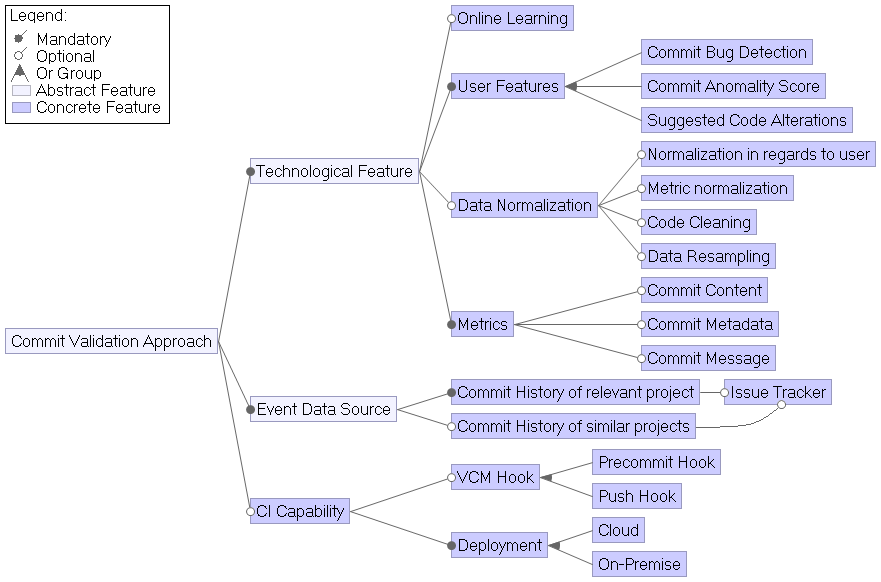
\includegraphics[width=15cm]{images/featuremodel}
	\caption{Featuremodel [TODO]}
\end{figure}

%Three categories have been specified for comparing Commit Validation approaches.
%TODO see in pdf view if the following is too long
For comparing Commit Validation approaches the three categories
\begin{itemize}
	\item Technological Features, 
	\item Event Data Source and
	\item CI Capability
\end{itemize}
have been defined.

The first category compares which \textit{Technological Features} approaches implement. The most important facette in this category are \textit{User Features}, which are features that a relevant to the end user of the approach. 
%Common user features are the detection of buggy commits and rating the anomality of commits.
More relevant to the performance of the approach are the facettes \textit{Metrics} and \textit{Data Normalization}. All approaches use some metrics to compare commit data, however the used metrics vary between the approaches.
%TODO correct grammar?
The later facette shows which normalization techniques are used in the approaches to further improve their classification performance.
\textit{Online-Learning} describes whether an approach is able to integrate analysis results made during production use into its analysis database, otherwise only the analysis results made on initial training data are considered. 

The \textit{Event Data Source} was also considered. This facette describes which sources of data are considered for training the classifier. All approaches are using the commit history of the repository for which new commits are being analyzed. Some approaches also used the commit history of similar repository or issue trackers which correspond to the repositories.
%TODO rename facettes in featuremodel from "...project" to "...repository".

Last % TODO correct wording?
the \textit{Capability for Continuous Capability} (or CI Capability) was considered. Because this paper focuses on Commit Validation, it is important how such an approach can be integrated into the commit process. As described in section \ref{sec:cvprocess}, VCM hooks are typical integration methods. The deployment of approaches is also interesting for practical usage, as a cloud based solutions can be incompatible with company guidelines.

%\begin{itemize}
%	\item Describe how relevant approaches differ from each other.
%	\item Derive list of criteria to compare Commit Validation approaches. For each criterium (roughly in one paragraph):
%	\begin{itemize}
%		\item Explain the criterium and what it means.
%		\item Discuss how the criterium is measured and derived from an Commit Validation approach.
%		\item Highlight the importance of this criterium in respect to comparing Commit Validation approaches.
%		\item Describe use cases for which this criterium is relevant.
%	\end{itemize}
%\end{itemize}

\subsection{Search Process}
\begin{itemize}
	\item Describe why CLEVER was used as starting point for research for this paper. \cite{Nayrolles2018}
	\item Describe how other approaches have been found based on CLEVER and how they match the papers scope as described in \ref{sec:scope}.
\end{itemize}

\subsection{Threads to Validity}
\begin{itemize}
	\item Discuss if there can be any biases when choosing and comparing Commit Validation approaches (See \cite{Kitchenham2004}).
	\item Describe how this paper made sure not to be biased.
\end{itemize}


\section{Comparison of Commit Validation Approaches}
\label{sec:comparison}

While the previous section has described the comparison schema, the results will now be presented. Section [TODO] specified categories with which the selected commit validation approaches have been categorized. The results are ordered using these categories. They are then presented in tabular form in table \ref{fig:classification}.

%TODO use \paragraph{title} per approach
\subsection{Purely Metric Based Approaches}

The approaches \textit{Commit Guru} by Rosen et. al. and \textit{Unusual Commits} by Goyal et. al. fall into the category of purely metric based approaches \cite{Rosen2015,Goyal2017}. They only rely on metrics that were directly derived from commits and used them to rate commits based on that. While Commit Guru works for any kinds of Git repositories, Unusual Commits only works for repositories hosted on GitHub \cite{Rosen2015,Goyal2017}.

Both approaches support Online Learning, thus every new commit after the initial training is taken into account for the analysis of later commits.
%Unusual Commits implemented more data normalization methods than Commit Guru. 
Unusual Commits also normalizes data in regards to user information by building a profile per project and per developer, thus user information is respected when analyzing commits. Both approaches did not mention that any other normalization techniques were used.
Both techniques also vary in their output: Unusual Commits is the only approach to not strictly categorize a commit as either buggy or not, instead it rates the likelyhood that a commit is \textit{unusual}, thus it differs from previous commits. Commit Guru outputs the same information as all other approaches, which is said categorization as buggy or not. \cite{Rosen2015,Goyal2017}

They also both use only the past commit history of the project which is analyzed as event data source, not any other data sources. Commit Guru is implemented in Python while Unusual Commits is realized in Java and R. It is also worth to mention that both implement a graphical user interface. Unusual Commits is implemented as Chrome Plugin which embeds classification results into the commit history on GitHub, while Commit Guru runs in a web application that lists a repositories analysis results. It also listens to new commits and automatically reanalyzes them and sends E-Mail notifications in response to the event, thus it shows CI capability in form of a Push Hook. Unusual Commits does not support and CI capabilities. Both are realized as free-to-use cloud applications. \cite{Rosen2015,Goyal2017}

Both approaches considered the metrics which regard the content of the commits, such as changed lines of code or the number of changed files. Commit Guru also considered the history of the commit, its purpose and information about the authoring developer, while Unusual Commits considered the length of the commit message, the time of commit and the changed file types. \cite{Rosen2015,Goyal2017}

%\subsection{Results for Approaches Based on Anomaly Detection}
%%TODO (TODO: I'm not sure yet if anomaly-based approaches differ from metric-based approaches enough to justify an additional subsection)
%\begin{itemize}
%\item Describe the results for approaches based on anomaly detection such as UnusualCommit (\cite{Goyal2017}).
%\end{itemize}

\subsection{Approaches based on Machine Learning}
\begin{itemize}
\item Describe the results for machine learning approaches.
\end{itemize}

\subsection{Approaches based on Code-Matching}
\begin{itemize}
\item Describe the results for machine learning approaches.
\end{itemize}

\subsection{Performance comparison}

When comparing Commit Validation approaches, the evaluation performance is an important point to consider. Due to the effort of this work and the fact that not all approaches are publicly available, an objective performance evaluation on all five approaches on a consistent dataset was out of scope for this paper. However, Nayrolles et. al. included an objective performance comparison between their approach and Rosen's approach \cite{Nayrolles2018}. In the same 
way, %TODO wording?
Yang et. al. included a performance comparison between their approach and Kamei's \cite{Yang2015}. While both use different datasets, it does give insights into how CLEVER compares to Commit Guru and how Deeper compares to Kamei's approach in regards to evaluation performance.

Table [TODO] describes the findings from Nayrolle's paper \cite{Nayrolles2018}, while table [TODO] describes the findings from Yang's paper \cite{Yang2015}.

\todo{Tables}

\todo{Describe tables}

%\begin{itemize}
%	\item Show Performance comparison tables
%	\item Describe tables
%\end{itemize}

\subsection{Comparison Results}
%\begin{itemize}
%	\item Table mapping all metrics/criteria (described in \ref{sec:scheme}) and all 5 approaches to results.
%\end{itemize}

The aforementioned results have been collected in Table \ref{fig:classification} where each of the described facettes map to specific values per identified Commit Validation approach.

\begin{figure}[H]
	\label{fig:classification}
	\centering
	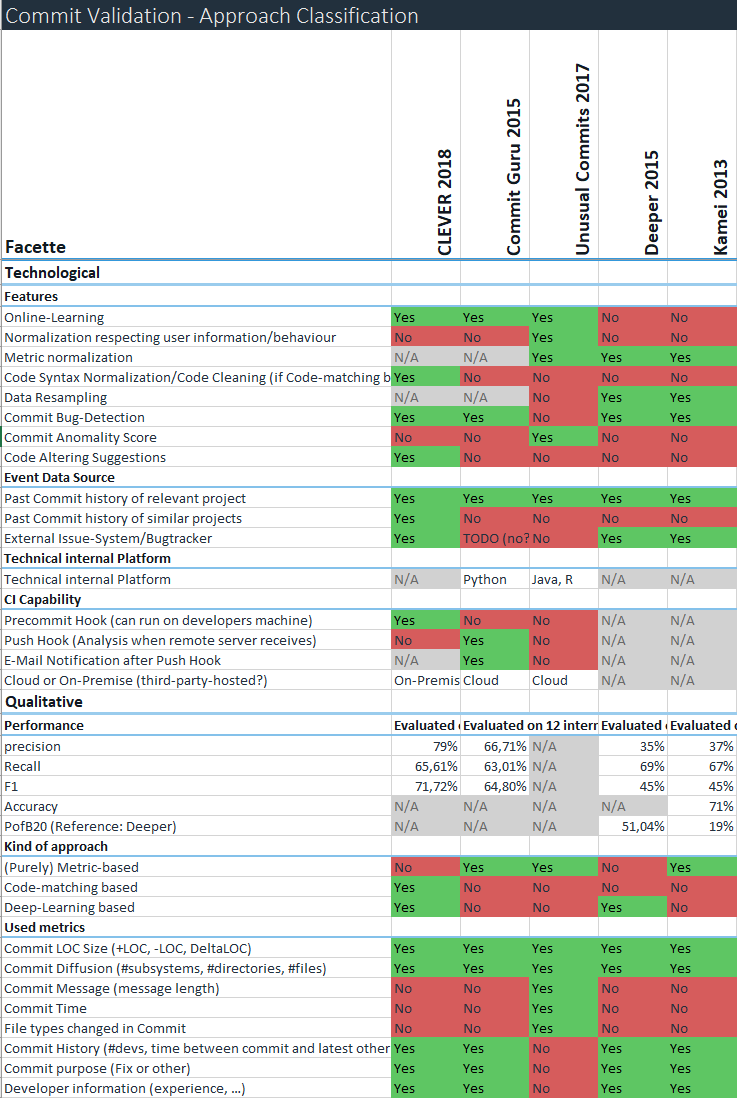
\includegraphics[width=15cm]{images/classification}
	\caption{Classification results [TODO]}
\end{figure}

\section{Discussion of Comparison Results}
\begin{itemize}
	\item Emphasize interesting findings from the results.
	\item Describe how performance was evaluated on the approaches and how their performance can be compared.
	\item Describe how the specified categories of Commit Validation techniques can be mapped to use cases.
	\item Outline how this mapping can be used to find an suitable Commit Validation technique for a new project.
\end{itemize}


\section{Related Surveys on Commit Validation}
\begin{itemize}
	\item Discuss and describe other surveys such as \cite{Kim2008,Catolino2019,Syed2019,Yang2016}.
	\item Highlight for each survey how its scope differs from the scope of this paper.
\end{itemize}


\section{Conclusions}

\subsection{Summary}
\begin{itemize}
	\item Give a short summary on the comparison scheme and which relevant criteria have been defined.
	\item Highlight interesting findings that were derived from the comparison results.
\end{itemize}

\subsection{Contributions}
\begin{itemize}
	\item Highlight the contributions that the proposed comparison scheme did to the scientific topic of Commit Validation.
	\item Discuss the relevance of the findings in regards to the scientific topic.
\end{itemize}

\subsection{Future Work}
\begin{itemize}
	\item Discuss relevant parts that have not been covered by this work.
	\item Highlight next steps to conduct to improve results.
\end{itemize}
